% \usepackage{amsmath,amssymb,amsfonts}
% \usepackage{algorithmic}
% \usepackage{graphicx}
% \usepackage[inline]{enumitem}
% \usepackage{tabularx}
% \usepackage{caption}
% \captionsetup{font=it}
% \usepackage[T2A,T1]{fontenc}
% % \usepackage[french]{babel}
% \usepackage{ragged2e}
% \usepackage{hyperref}
% \usepackage{footmisc}
% \usepackage{booktabs}
% \usepackage{smartdiagram}
% \usepackage{setspace}
% \usepackage{textcomp}
% \usepackage{xcolor}
% \def\BibTeX{{\rm B\kern-.05em{\sc i\kern-.025em b}\kern-.08em
%     T\kern-.1667em\lower.7ex\hbox{E}\kern-.125emX}}
% \usepackage{cite}
% \usepackage{amsmath}
% \newcommand{\probP}{\text{I\kern-0.15em P}}

% \usepackage{etoolbox}
% \patchcmd{\thebibliography}{\section*{\refname}}{}{}{}


% \newcommand{\old}[1]{\textcolor{orange}{#1}}
% \newcommand{\rem}[1]{\textcolor{red}{#1}}
% \newcommand{\todo}[1]{\textcolor{orange}{\newline \textit{\textbf{TODO:} #1}} \newline \newline }


\section{Introduction}

Le développement de l'<<~Internet of Things~>> et de l'<<~Internet of Battle Things~>>  a entrainé une augmentation de la surface d'attaque des systèmes en réseau.
%permettant à des attaquants de s'y introduire en ciblant les nœuds les plus faiblement défendus.
Tenant compte de ce contexte, le groupe de travail <<~AICA IWG~>>\footnote{Ce groupe de travail (voir \url{https://www.aica-iwg.org/}) s'appuie sur les résultats du \textit{Research Task Group IST-152} de l'OTAN qui a travaillé sur le concept des <<~Intelligent, Autonomous and Trusted Agents for Cyber Defense and Resilience~>>.} développe des travaux sur les agents AICA (Autonomous Intelligent Cyber-defence Agent).
Un agent est par définition une entité autonome capable de percevoir son environnement local grâce à des capteurs, et d'agir sur cet environnement à l'aide d'effecteurs\cite{russell1995modern}.
L'agent AICA doit pouvoir être déployé sur un système hôte pour détecter, identifier et caractériser des anomalies/attaques, élaborer et piloter l'exécution de contre-mesures et dialoguer avec l'extérieur. À cette fin, il est conçu comme proactif, discret et capable d'apprendre.


L'agent AICA peut être conçu comme un Système Multi-Agent (SMA). Le paradigme multi-agent offre des moyens de gérer l'ouverture, le passage à l'échelle et l'autonomie du système hôte en déléguant différents aspects de la cyber-défense à différents agents. L'agent AICA  est alors un système collectif décentralisé et distribué d'agents cyber-défenseurs déployés au plus près des composants du système\cite{ieeesp_KottT20}.

Notre problématique consiste à définir l'organisation du SMA qui permettrait de répondre à des besoins de cyber-défense compte tenu des contraintes d'un environnement de déploiement en réseau.


\section{SMA de Cyber-défense}

Nous appelons \textbf{cyber-défense} l'ensemble des activités entreprises lorsqu'une cyber-attaque est détectée et qu'il est nécessaire de réagir\cite{theron_autonomous_2021}. Ces activités sont décrites dans le cadre du <<~P3R3 Resilience Engineering Framework~>>\cite{Theron2013P3R3} et sont regroupées en trois fonctions de cyber-défense :

\textit{R1 - Detect and alarm} : détection des cyber-attaques  et déclenchement des mécanismes de réponse;

\textit{R2 - Respond and restore} : mise en œuvre et suivi des réponses apportées aux cyber-attaques et à la restauration des niveaux de services/activités minimaux. La gestion de la crise provoquée par l'attaque est au cœur de cette fonction;

\textit{R3 - Recover and rebound} : rétablissement des parties endommagées du système à défendre et traitement final des conséquences. Ce point inclut une phase d'apprentissage permettant l'amélioration du système de cyber-défense.


Nous nommons \textbf{objectifs de cyber-défense}, tous les objectifs impliquant la mise en œuvre d'une ou plusieurs des fonctions de cyber-défense.

Dans un \textbf{SMA de cyber-défense}, plusieurs agents atteignent un objectif global de cyber-défense par le comportement collectif résultant de la réalisation de sous-objectifs individuels et/ou de mécanismes locaux\cite{jamont2015meeting}. Des exemples de tels sous-objectifs pourraient être la détection des intrusions, la mise en œuvre d'un plan de récupération, la restauration d'une image, la redirection des ports\dots


Prenant appui sur un rapprochement des notions de SMA et cyber-défense dans la littérature, nous avons considéré chacun des travaux selon les fonctions de cyber-défense qu'il couvre.
Nous avons constaté que la plupart des objectifs de cyber-défense des SMA se concentrent principalement sur la détection d'anomalies et d'intrusions (plus de 50\% des travaux de notre revue complète se focalisent sur la fonction R1).

Pour chacun de ces mêmes travaux, nous nous sommes aussi intéressés aux caractéristiques principales de l'organisation et de l'environnement de déploiement.
Nous constatons qu'indépendamment des objectifs de cyber-défense, l'organisation centralisée et/ou hiérarchique est la plus répandue parmi les SMA de cyber-défense étudiés.

\noindent

La centralisation des données acquises de l'environnement, en un seul point, favorise de meilleures performances pour l'analyse de la situation globale et le contrôle du système de cyber-défense. Ces types d'organisation semblent moins facilement s'appliquer pour des réseaux dynamiques, mais sont répandus sur des systèmes de taille moyenne avec des contraintes connues\cite{vasilomanolakis2015taxonomy}.

\noindent

% Les organisations alternatives de type décentralisé prennent davantage en compte l'incertitude des cyber-attaques en laissant l'autonomie aux agents de s'organiser sans attentes d'organisation définies a priori.Le <<~Artificial Immune System~>> \cite{morteza2015method} ou la <<~Ant-Based Cyber Security~>> \cite {haack2011ant} en sont des exemples, mais restent peu établies en tant que solution de cyber-défense.

Les organisations alternatives identifiées comme décentralisées prennent davantage en compte l'incertitude des cyber-attaques en laissant l'autonomie aux agents de s'organiser sans atteindre d'organisation définies a priori. Cependant, elles restent peu établies en tant que solution de cyber-défense.


Cette revue a permis d'identifier de premiers mécanismes sous-jacents à un SMA de cyber-défense. Cependant, la diversité (des objectifs, des environnements, des architectures d'agents, des protocoles d'interaction\dots) des SMA de cyber-défense disponibles rend l'appréciation générale des organisations difficile sans cadre commun.
Il apparaît nécessaire d'avoir un modèle permettant de modéliser le système hôte sur lequel sont déployés des agents attaquants et défenseurs.

\section{Établissement d'une modélisation}

\textbf{Environnement de déploiement des agents}\qquad Reprenant un cas d'usage de l'AICA\cite{theron_autonomous_2021}, nous nous intéressons à un environnement réseau constitué de \textit{nœuds} sur lesquels des \textit{agents} d'attaque et de défense peuvent être déployés pour les observer et agir. Ces nœuds peuvent être décrits par un ensemble de \textit{propriétés} liées aux processus, au système de fichier, au système d'exploitation, à l'architecture matérielle, etc.
Les \textit{observations} et \textit{actions} des agents sont conditionnées par leurs propriétés propres (dont les propriétés connues par eux) et une éventuelle non-certitude. Par exemple, la lecture d'un fichier donné ou une redirection des ports peut nécessiter un niveau de privilège élevé; ou encore, la réception de données d'un capteur physique n'est pas assurée en tout temps.
Chaque agent appliquant une/des action(s), modifie les propriétés d'un ou plusieurs nœuds. Cela change l'état de l'environnement induisant un éloignement/rapprochement des agents de leur(s) objectif(s).

\textbf{Vers une modélisation de l'environnement}\quad Les caractéristiques de cet environnement de déploiement l'inscrivent comme un cas spécifique d'un <<~Partially Observable Stochastic Game~>> (POSG) et plus spécifiquement d'un <<~Decentralized Partially Observable Markov Decision Process~>> (Dec-POMDP).
Les POSGs et les Dec-POMDPs sont tous les deux des cadres de modélisation mathématique de problèmes de prise de décision dans lesquels les agents interagissent entre eux et dans un environnement stochastique\cite{beynier2010}. Dans un POSG, un groupe d'agents interagit avec un environnement stochastique et partiellement observable. Chaque agent agit en fonction de ses propres observations et d'une politique locale. Les agents peuvent avoir des objectifs différents et le jeu est généralement supposé non coopératif\cite{jk2020}.
Dans un Dec-POMDP, les agents doivent coordonner leurs actions pour atteindre un objectif commun en étant capables de communiquer\cite{bernstein2013}.

\

\textbf{Modélisation Dec-POMDP} \quad Notre modèle Dec-POMDP intègre la notion de propriétés de nœud modifiables par des actions qu'appliquent les agents. Adoptant le jeu séquentiel simple du modèle <<~Agent Environment Cycle~>>\cite{jk2020}, dans notre modèle, chaque itération se déroule de la façon suivante:
\begin{enumerate*}[label=\roman*),itemjoin={;\quad}]
  \item Un agent choisit une action à partir des observations précédentes (propriétés connues) selon une fonction de comportement
  \item L'environnement est mis à jour par une fonction de transition dépendant de l'état précédent et de l'action prise par l'agent (changement de propriétés une fois la pré-condition satisfaite)
  \item Une observation est renvoyée à l'agent en se basant sur l'état actuel (propriétés connues de l'agent) et l'action associée selon une fonction d'observation. Une récompense basée sur l'évaluation des métriques recueillies pour cet état courant est également envoyée à l'agent.
\end{enumerate*}

Nous posons les éléments relatifs aux propriétés des nœuds, agents et actions de l'environnement suivants :

$Ag = \{ag_1,..,ag_{|Ag|}\}$ : L'ensemble des agents

$P_j = \{ p_1, .., p_{|P_{j}|} \}$ : L'ensemble des propriétés du nœud $j$ ($j \in N$). Par exemple, les identifiants des processus en cours d'exécution, les fichiers disponibles dans un dossier, le type de système d'exploitation, etc.

$P = \{ P_1, .., P_{|P|} \}$ : L'ensemble des propriétés de tous les nœuds.

$Kb: P \times Ag \rightarrow P_Ag, P_{Ag} \subset P$ : Donne les propriétés connues par un agent.

$Action : \mathcal{P}(P) \rightarrow P$ : L'ensemble des relations qui associent une pré-condition de propriétés à un à un ensemble de propriétés nouvelles. Par exemple, les propriétés <<~l'agent X est root~>>, <<~l'agent X accède à Vim~>> et <<~l'agent X connaît l'emplacement du fichier .bashrc~>> forment une pré-condition pour y associer les propriétés précédentes en plus de la propriété <<~fichier .bashrc est modifié par agent X~>>.

$Metrics: P \rightarrow \mathbb{R}^{n}$ : Donne les métriques associées à un ensemble de propriétés. Par exemple, le nombre de nœuds encore actifs, le nombre de déplacements latéraux, etc.

\

Reprenant la description formelle d'un Dec-POMDP\cite{OliehoekA16}, nous proposons le modèle suivant :

$S = \{s_1, ..s_{|S|}, s_{i} \subseteq P\}$ : L'espace des ensembles de propriétés possibles.

$A_i = \{a_{i}^{1},..,a_{i}^{|A_{i}|}\} \: with \: a_{i}^k \in Action \: (with \: k \in {1, .., |A_i|})$ : L'ensemble des actions pour l'agent $i$.

$T(s,a,s') = \probP{(s'|s,a)}$ : La probabilité de transition d'un état; et $\probP{(s'|s,a)} = 0$ si $s'$ ne satisfait pas la pré-condition de $a$.

$R: S \times A \rightarrow N = Eval \circ Metrics \circ Next$ : La fonction de récompense avec $Eval: \mathbb{R}^n \rightarrow \mathbb{R}$, associant les métriques à une récompense; et $Next: S \times A \rightarrow S$, donnant l'état induit par une action.

$\Omega_i \subset Im(Kb) \subset P$ : L'ensemble des observations pour l'agent $i$. Par exemple, le contenu d'un fichier, la sortie de logs d'une commande, le résultat d'un scan des ports, etc.
$O(s',a,o) = \probP{(o|s',a)}$ : La probabilité qu'un agent observe un ensemble de propriétés. Avec $\probP{(o|s',a)} = 1$ si l'état $s'$ contient les propriétés de $o$.
Par exemple, un agent joue l'action <<~l'agent X lit un fichier de log", il résulte un nouvel état dont une propriété appartenant à la connaissance de l'agent X est <<~le contenu du fichier de log 'abc' est connu de l'agent X". L'observation <<~le contenu du fichier de log est 'abc'~>> sera donc retourné à l'agent X.

\



% \singlespacing




% \begin{figure}
%     \centering
% \begin{center}
%   \makebox[\textwidth]{\includegraphics[width=\paperwidth]{figures/schéma_tour_details_exemple.png}}
% \end{center}
% \caption{Détails d'un tour}
%     \label{fig:detail_tour_exemple}
% \end{figure}


% \section{Approches de résolution}

% Résoudre un Dec-POMDP implique de trouver une politique pour chaque agent qui maximise la somme des récompenses individuelles obtenues par chaque agent\cite{jk2020}. Il s'agit d'un problème difficile en raison du grand espace d'état et du besoin de coordination entre les agents. Différentes approches ont été proposées, notamment la programmation dynamique, la << value iteration >>, la << policy iteration >>, l'apprentissage par renforcement, << Distributed Constrained Optimization Problem >>, les méthodes de Monte Carlo et les méthodes de la théorie des jeux telles que l'équilibre de Nash\cite{OliehoekA16}.


\section{Vers une implémentation}

Parmi les simulateurs que nous avons identifiés pour implémenter le modèle Dec-POMDP, aucun ne permet de couvrir à la fois la prise en compte d'un environnement cyber multi-agent selon le modèle Dec-POMDP et le besoin d'accessibilité du code (code ouvert) permettant de façon simple l'implémentation des agents attaquants et défenseurs.
Cependant, nous avons identifié le framework Python <<~PettingZoo~>>, conçu pour permettre l'implémentation d'un Dec-POMDP\cite{jk2020}. Il fournit un framework où le concepteur dispose d'outils pour faciliter la mise en place de l'espace des observations, des actions, de la gestion des agents à chaque tour et des récompenses associées\cite{jk2020}.

% PettingZooo est en fait une adaptation multi-agent de <<~Open AI Gym~>>~\cite{openAIGym2016}, plateforme d'apprentissage par renforcement pour un seul agent et sur lequel a été développé l'environnement <<~CyberBattleSim~>>\cite{cyberbattlesim}. Cet environnement de nœuds en réseau sur lequel un attaquant agit pour atteindre son objectif, est une source d'inspiration pour mettre en place un environnement similaire reposant sur PettingZoo.

Le développement de notre modèle avec PettingZoo, permet de proposer le simulateur <<~Multi Cyber Agent Simulator~>> (MCAS)\cite{MCASWebsite}. Un aperçu de l'interface de ce simulateur est présenté Figure~\ref{fig:interface_simulateur}. En l'état actuel du développement, ce simulateur permet de charger/sauvegarder un environnement, de lancer l'exécution des agents de cet environnement en mode tour par tour via le terminal (en bas à droite de la Figure~\ref{fig:interface_simulateur}). Il permet aussi d'afficher les propriétés des nœuds de l'environnement sous format \textit{json} (partie gauche de la Figure~\ref{fig:interface_simulateur}) et visualiser l'environnement sous forme d'un graphe et l'affichage des métriques.


\begin{figure}
  \centering
  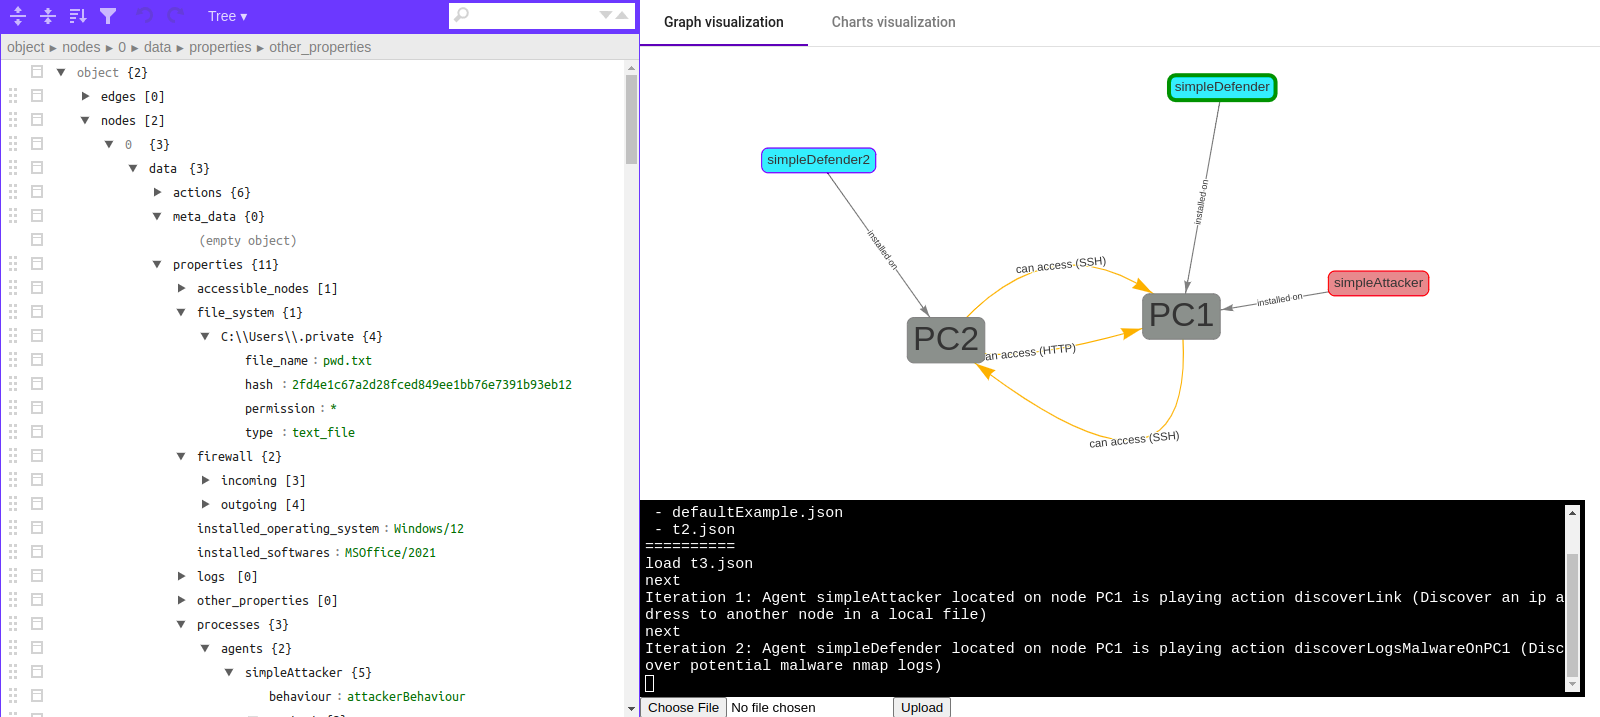
\includegraphics[width=\linewidth]{figures/interface_MCAS.png}
  \caption{Aperçu de l'interface du simulateur}
  \label{fig:interface_simulateur}
\end{figure}

\section{Conclusion}
Un SMA de cyber-défense déployé sur un système hôte en réseau permettrait de relever les défis liés à la complexité et la rapidité de cyber-attaques. Une première étude bibliographique donne un aperçu des liens entre l'environnement de déploiement, les objectifs et l'organisation adoptée par le concepteur du SMA de cyber-défense.
Montrant des limites pour une compréhension générale, nous proposons une modélisation sous la forme d'un Dec-POMDP fournissant un cadre théorique général pour notre problématique et bénéficiant de plusieurs approches algorithmiques de résolution établies. La mise en œuvre de ce modèle prend la forme d'un simulateur pensé pour être utilisé dans le futur avec un protocole expérimental visant à évaluer et tirer des recommandations sur l'organisation d'un SMA de cyber-défense.
